% fig_domain_map.tex -- linear domain map of aRES (UC5), two annotation tracks.
% Boundaries: docs/05 section 1.1 (PAE blocks) and docs/07 section 1 (Zn ribbon).
% Coordinates are in residue units: the x unit vector is set to 0.0295 cm.
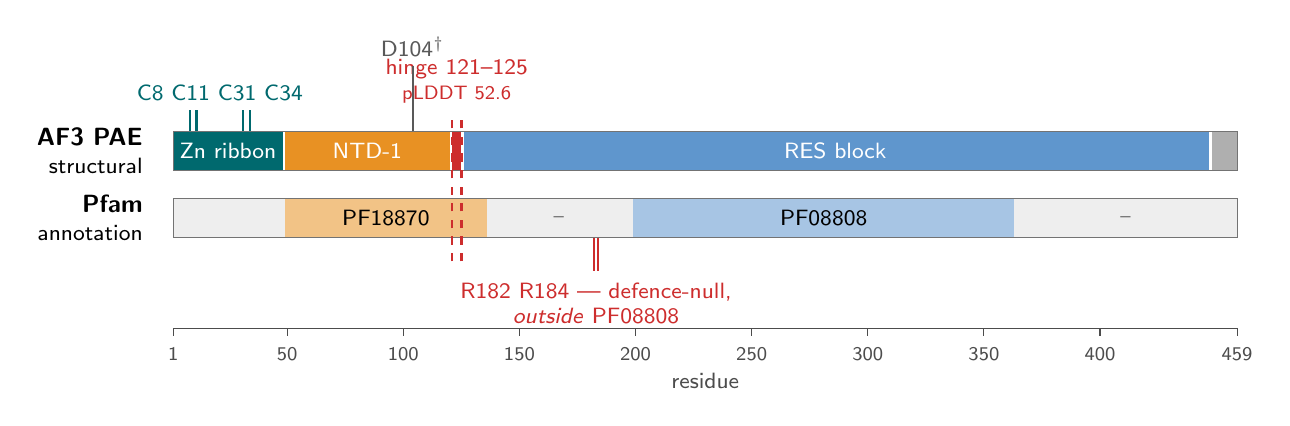
\begin{tikzpicture}[x=0.0295cm, y=1cm, font=\sffamily\small]

  \definecolor{znribbon}{RGB}{0,105,110}
  \definecolor{ntd1col}{RGB}{232,145,35}
  \definecolor{hingecol}{RGB}{205,45,45}
  \definecolor{rescol}{RGB}{95,150,205}
  \definecolor{tailcol}{RGB}{175,175,175}
  \definecolor{unassigned}{RGB}{238,238,238}

  % ---------- track 1: AF3 PAE structural blocks ----------
  \node[anchor=east, align=right] at (-8, 1.10)
    {\textbf{AF3 PAE}\\[-1pt]\footnotesize structural};

  \fill[znribbon]  (1,0.85)   rectangle (48,1.35);
  \fill[ntd1col]   (49,0.85)  rectangle (120,1.35);
  \fill[hingecol]  (121,0.85) rectangle (125,1.35);
  \fill[rescol]    (126,0.85) rectangle (447,1.35);
  \fill[tailcol]   (448,0.85) rectangle (459,1.35);
  \draw[black!55, line width=0.3pt] (1,0.85) rectangle (459,1.35);

  \node[white]        at (24.5,1.10) {\footnotesize Zn ribbon};
  \node[white]        at (84.5,1.10) {\footnotesize NTD-1};
  \node[white]        at (286,1.10)  {\footnotesize RES block};

  % ---------- track 2: Pfam ----------
  \node[anchor=east, align=right] at (-8, 0.25)
    {\textbf{Pfam}\\[-1pt]\footnotesize annotation};

  \fill[unassigned] (1,0)   rectangle (459,0.50);
  \fill[ntd1col!55] (49,0)  rectangle (136,0.50);
  \fill[rescol!55]  (199,0) rectangle (363,0.50);
  \draw[black!55, line width=0.3pt] (1,0) rectangle (459,0.50);

  \node at (92.5,0.25) {\footnotesize PF18870};
  \node at (281,0.25)  {\footnotesize PF08808};
  \node[black!55] at (167,0.25) {\scriptsize --};
  \node[black!55] at (411,0.25) {\scriptsize --};

  % ---------- the hinge discrepancy ----------
  \draw[hingecol, line width=0.9pt, dashed] (121,-0.30) -- (121,1.55);
  \draw[hingecol, line width=0.9pt, dashed] (125,-0.30) -- (125,1.55);
  \node[hingecol, anchor=south, align=center] at (123,1.58)
    {\footnotesize hinge 121--125\\[-2pt]\scriptsize pLDDT 52.6};

  % ---------- zinc-site cysteines ----------
  \foreach \r in {8,11,31,34}{%
    \draw[znribbon, line width=0.8pt] (\r,1.35) -- (\r,1.62);}
  \node[znribbon, anchor=south, align=center] at (21,1.62)
    {\footnotesize C8 C11 C31 C34};

  % ---------- D104 ----------
  \draw[black!65, line width=0.7pt] (104,1.35) -- (104,2.18);
  \node[black!65, anchor=south] at (104,2.18) {\footnotesize D104$^{\dagger}$};

  % ---------- R182 / R184 fall OUTSIDE the Pfam RES call ----------
  \foreach \r in {182,184}{%
    \draw[hingecol, line width=0.8pt] (\r,0) -- (\r,-0.42);}
  \node[hingecol, anchor=north, align=center] at (183,-0.45)
    {\footnotesize R182 R184 --- defence-null,\\[-2pt]
     \footnotesize \emph{outside} PF08808};

  % ---------- residue axis ----------
  \draw[black!70] (1,-1.15) -- (459,-1.15);
  \foreach \r in {1,50,100,150,200,250,300,350,400,459}{%
    \draw[black!70] (\r,-1.15) -- (\r,-1.25);
    \node[anchor=north, black!70] at (\r,-1.27) {\scriptsize \r};}
  \node[anchor=north, black!70] at (230,-1.60) {\footnotesize residue};

\end{tikzpicture}
